\documentclass[aspectratio=169]{beamer}
\usepackage{amsmath, amssymb, amsfonts, amsthm}
\usepackage{lmodern}
\usepackage{cancel}
\usepackage[output-complex-root=j]{siunitx}
\usepackage[american, nooldvoltagedirection]{circuitikz}
\usepackage{bm}
\usepackage{listings}
\usepackage{graphicx}
\usepackage{hyperref}

\usetheme{Berkeley}
\usefonttheme[onlymath]{serif}
\AtBeginSection[]{
    \begin{frame}
    \vfill
    \centering
    \begin{beamercolorbox}[sep=8pt,center,shadow=false,rounded=false]{title}
    \usebeamerfont{title}\insertsectionhead\par
    \end{beamercolorbox}
    \vfill
    \end{frame}
}

\newcommand{\N}{\mathbb{N}}
\newcommand{\Z}{\mathbb{Z}}
\newcommand{\Q}{\mathbb{Q}}
\newcommand{\R}{\mathbb{R}}
\renewcommand{\C}{\mathbb{C}}
\newcommand{\tpose}[1]{\left[#1\right]^{\! \top} \!\!}

\title{EECS 16B CSM}
\author{Bryan Ngo}
\date{2020-11-15}
\institute{UC Berkeley}

\begin{document}

\begin{frame}
    \maketitle
\end{frame}

\begin{frame}
    \frametitle{Logistics}

    \begin{itemize}
        \item Linear algebra review
        \item SVD review
        \item Applications of SVD
        \item PCA
    \end{itemize}
\end{frame}

\section{Principal Component Analysis}

\begin{frame}
    \frametitle{Motivation}

    \begin{itemize}
        \item used for statistical analysis
        \item clustering
        \item correlation
    \end{itemize}
\end{frame}

\begin{frame}
    \frametitle{How to PCA}

    Given \(\bm{A} \in \R^{n \times m}\), \(n\) measurements with \(m\) samples,
    \begin{enumerate}
        \item find \(\overline{n_i}\) to center \(\bm{A}\) around mean
        \item find SVD \(\widetilde{\bm{A}} = \bm{U \Sigma V}^\top\)
        \item plot eigenvectors/principal components \(\bm{v}_1, \bm{v}_2\) against centered points
        \item data is scaled by \(\sigma_1, \sigma_2\)
        \item more stretched along vector \(\implies\) larger correlation
    \end{enumerate}
\end{frame}

\begin{frame}
    \frametitle{Visualization}

    \centering
    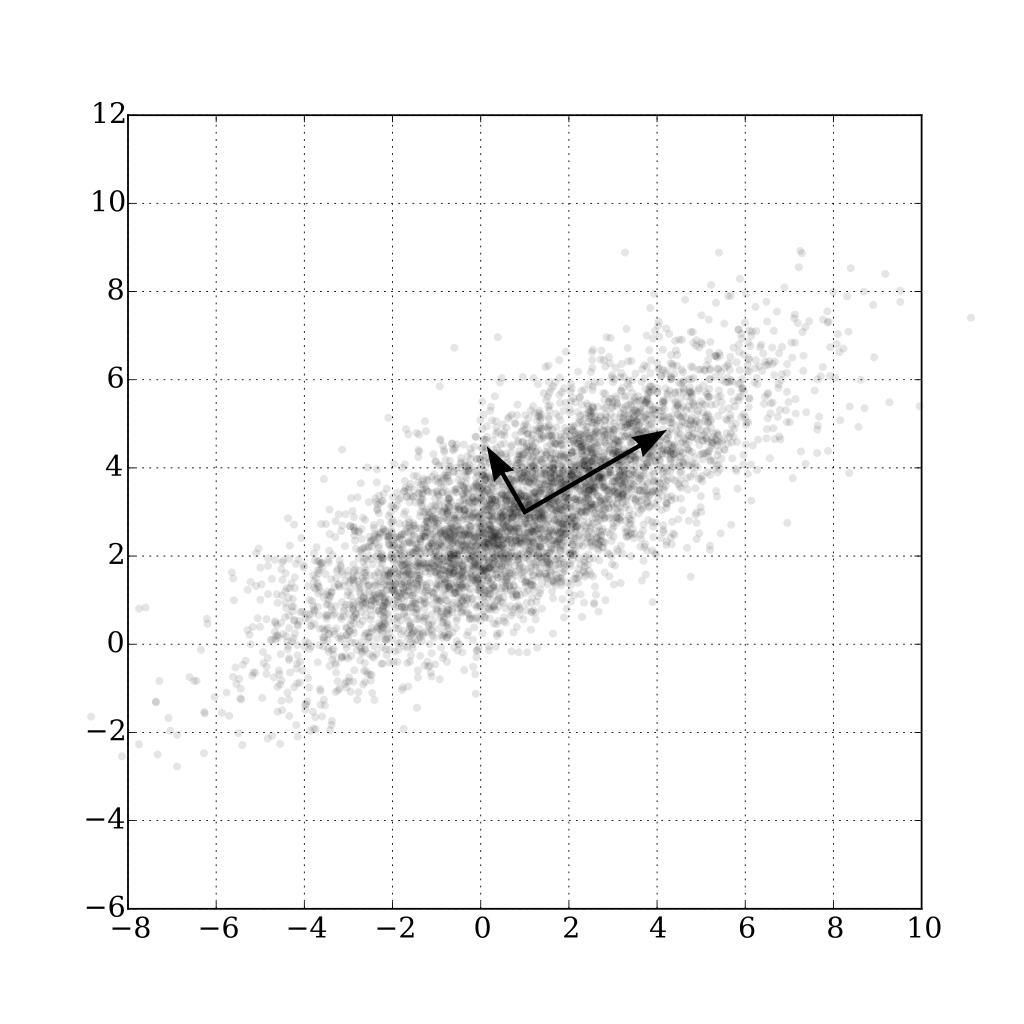
\includegraphics[height=0.9\textheight]{1024px-GaussianScatterPCA.svg.png}
\end{frame}

\end{document}
